\chapter{Fundamentals-Theory for this approach to reach 5G}
\label{ch:fundamentals}
\textit{Presentation of the theoretical basis required for an understanding of your work. Do not begin with Newton's laws or Maxwell's equations: imagine that the reader is a competent engineering professor, but not necessarily in your field of expertise. Do not bother to discuss any theory that you do not employ in later sections.}
In the following some fundamentals are described shortly.
\section{Concept of Software-defined radio}
The concept of software-defined radio is adapted to deal with the old problems of mobile communication. The idea is to bring the digital domain as close as possible to the RFFE. The reason is digital filtering, data processing is more efficient, easier, less complex, has less cost, and so on. The main problem of this approach is the energy consumption based on an inefficient ADC/DAC. However the concept is very helpful for future designs of an digital front end. The Software-defined radio has the advantage, that it is adaptiv for future software changes. the hardware is still the same, only the firmware has to be upgraded. broad spectrum of signal can be received with this architecture. from nearly DC to 2 GHz. For future mobile communication standards, the frequency range has to deal with frequencies beyond 2 GHz up to 6 GHz. Nowadays IEEE802.11ac standard is located at 5GHz. Based on this concept a digital-analog converter is designed to deal with a higher bandwith than other devices nowadays. The DAC is used in the transmission path of the design.
%\section{An approach to reach the desired high speed for the digital-to-analog converter: The Riemann Pump}
\section{Idea of the Riemann Pump}
The Riemann Pump is a arbitrary waveform generator which is controlled through a digital input control voltage.
In fact of the conversion from digital to analog signals this can be seen as a \gls{ab:dac}.
% By applying a digital input voltage of \SI{5}{\volt} a arbitrary wave form can be generated.
The idea of a Riemann Pump is based on the concept of a charge pump, as the name suggests.
% The concept is based on the idea to charge a capacitor at the output.
With this concept it is possible to realize this \gls{ab:dac} as close as possible to the RF front end.
Therefore there is no intermediate step of signal processing which decrease the latency.
The benefit of this concept is to realize this \gls{ab:dac} as close as possible to the RF front end without an intermediate step of
that the output capacitor can be realized with a pre power amplifier, because that got a capacitive input characteristic.
Therefore the signal can be directly amplified and transmitted.
The Riemann Pump, named after the mathematician Riemann, who founded the Riemann Integral, is a special charge pump. A charge pump as the name suggests pumps electrons into a capacitve load. Across the load capacitance a voltage is created. By adjusting the switches for up or down the voltage can be adjusted, as seen in Fig. \ref{fig:ChargePump}. 

\begin{figure}[ht]
	\centering
  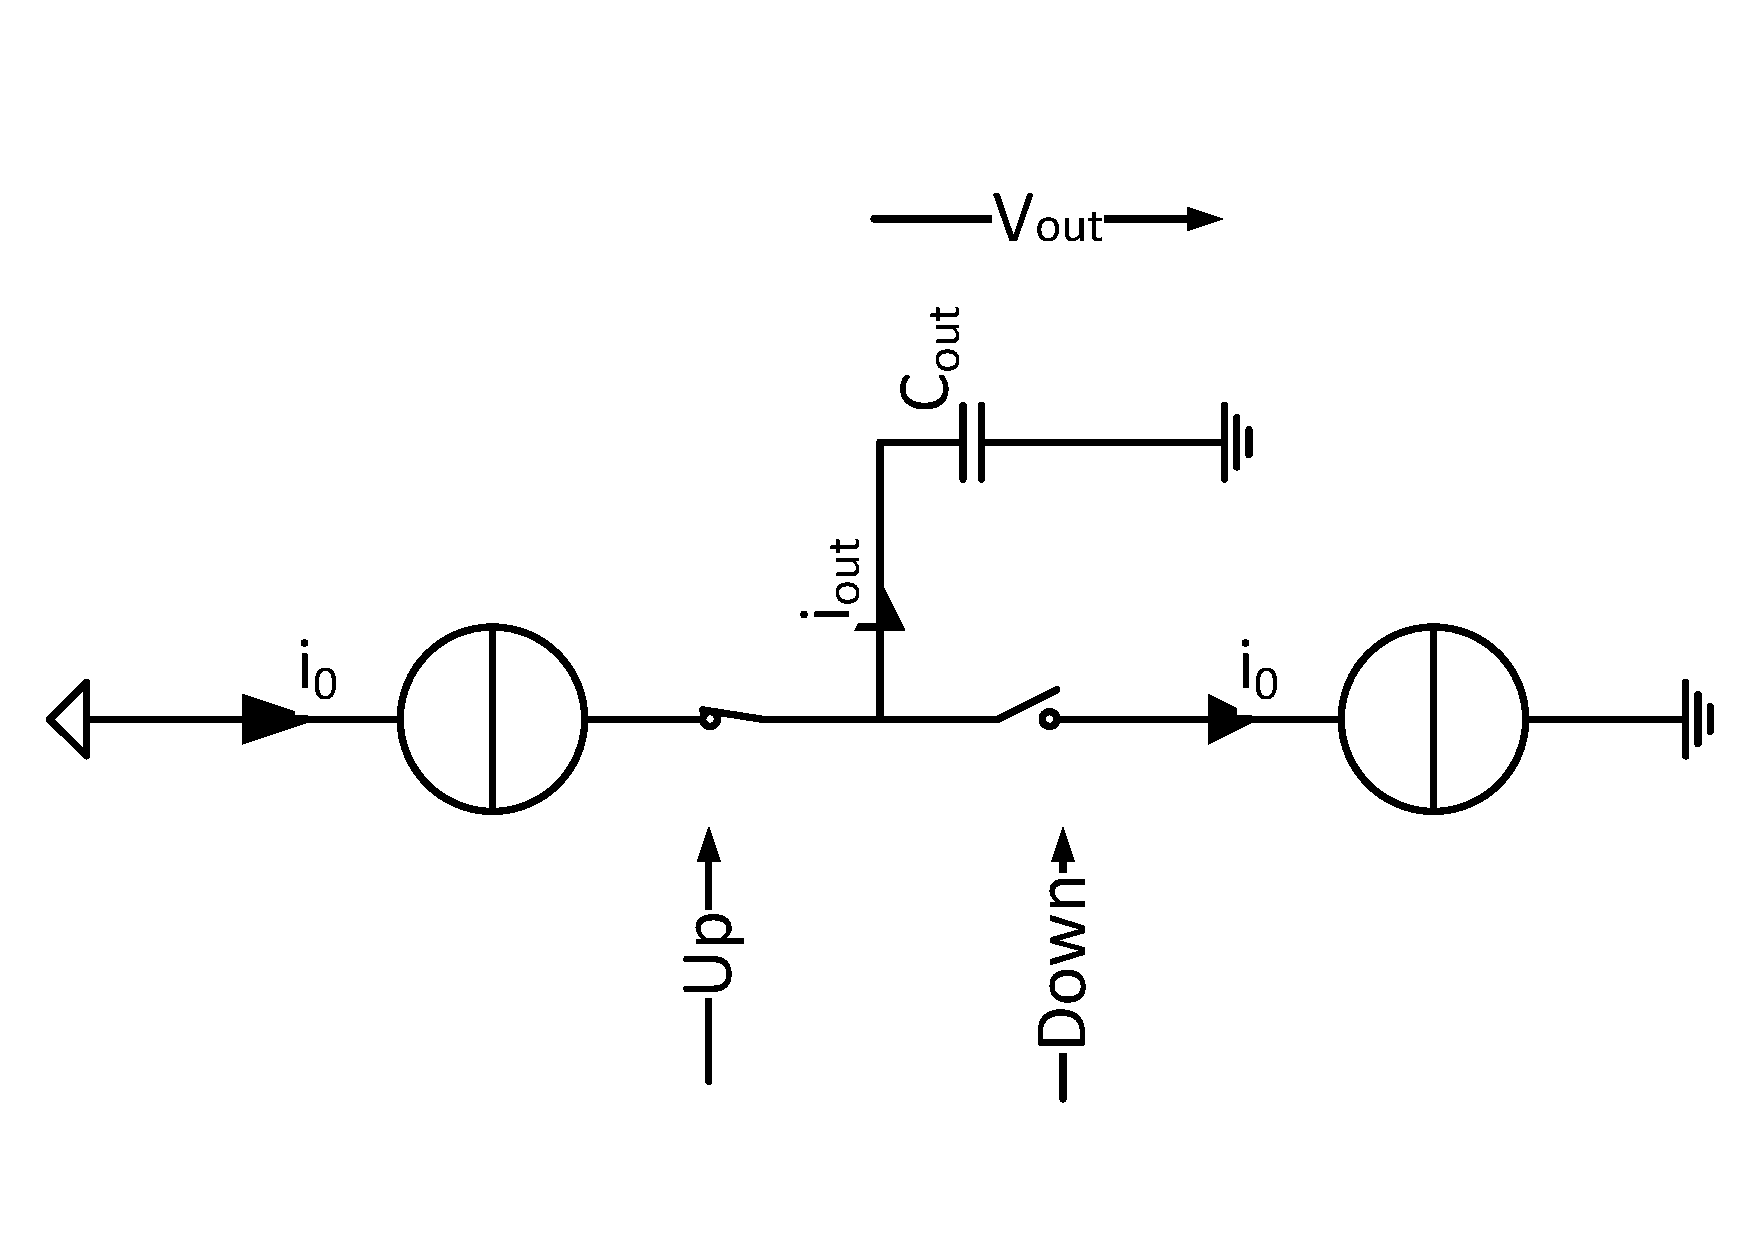
\includegraphics[width=0.5\textwidth, angle = 270]{ChargePump.pdf}
	\caption{scheme of a charge pump; works like a Riemann Pump with one-bit resolution}
	\label{fig:ChargePump}
\end{figure}

\begin{equation}
	V_{out} = \frac{1}{C_{out}}{ \int_0^T \! i_{out}(t) \, \mathrm{d}t} , \hspace{1cm} T = \frac{2*OSR}{f_{sample}}
\end{equation}

The Riemann Pump is a digital-to-analog converter based on the concept of a charge pump. A few charge pumps with different sized sources in parallel shows the concept of this fast digital to analog converter. With the ability to control the switches really fast, because of the use of GaN25 technology, which have a high transition frequency, a high bandwidth is reached.

\begin{figure}[ht]
	\centering
  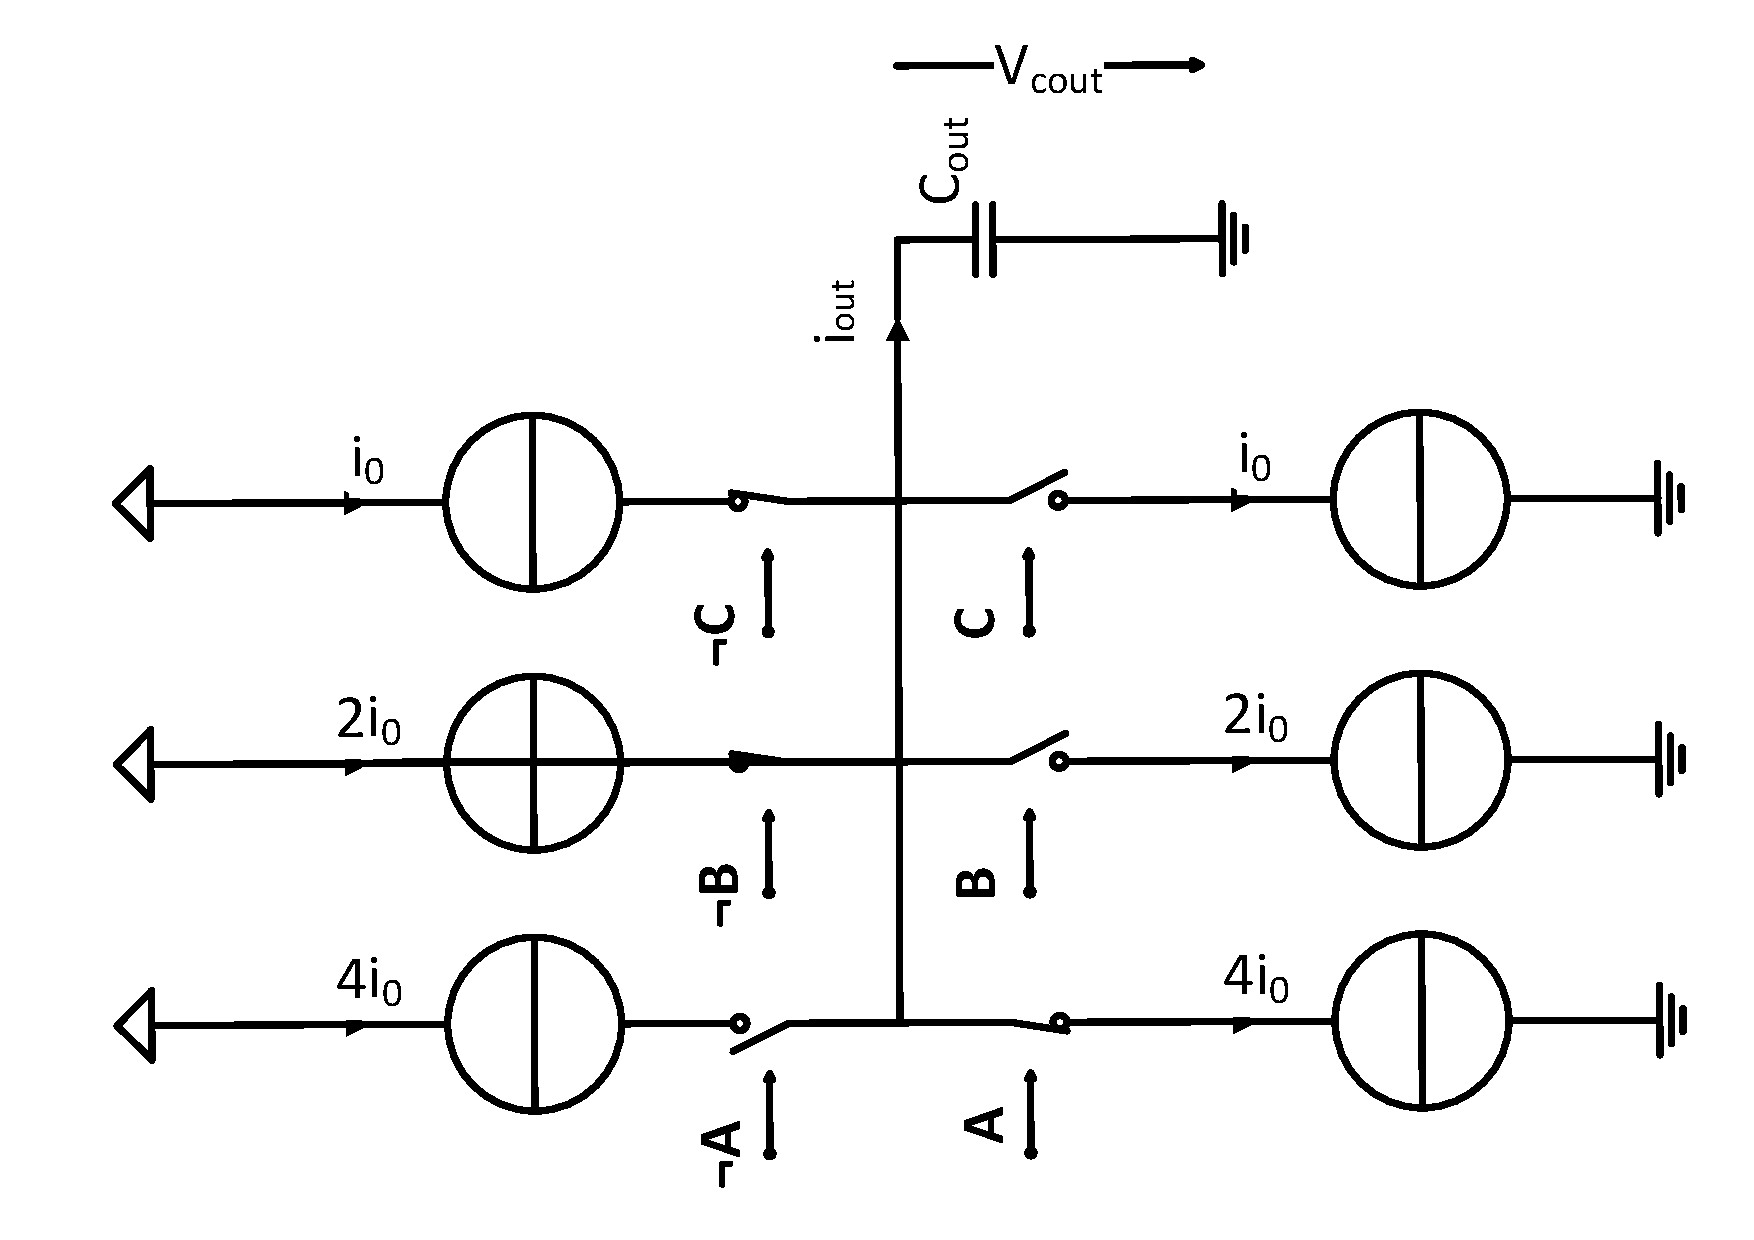
\includegraphics[width=0.5\textwidth, angle = 270]{RP_concept.pdf}
	\caption{Concept of the Riemann Pump with three-bit resolution}
	\label{fig:RiemannPumpConcept}
\end{figure}

 The working principle is to integrate a current into a capacitive load, this integration is based on Riemann Integral, where the name come from. This integration converts the current into a voltage. This output voltage can be applied to the input of a power amp and then to the antenna to propagate it. The current, which charges the capacitive input impedance of the power amp, is controlled by a digital code. A fixed set of slopes, represents the different current sources. A desired signal in the time-domain is generated with MatLab. This signal can consist of many different signals (different carriers and modulation types). This signal is sampled with the given set of slopes. The minimization of the error leads to the Riemann Code. With this Riemann Code (digital) the driver circuit is controlled. This leads to an analog signal formed by the digital input signal. 
 
\begin{figure}[ht]
	\centering
  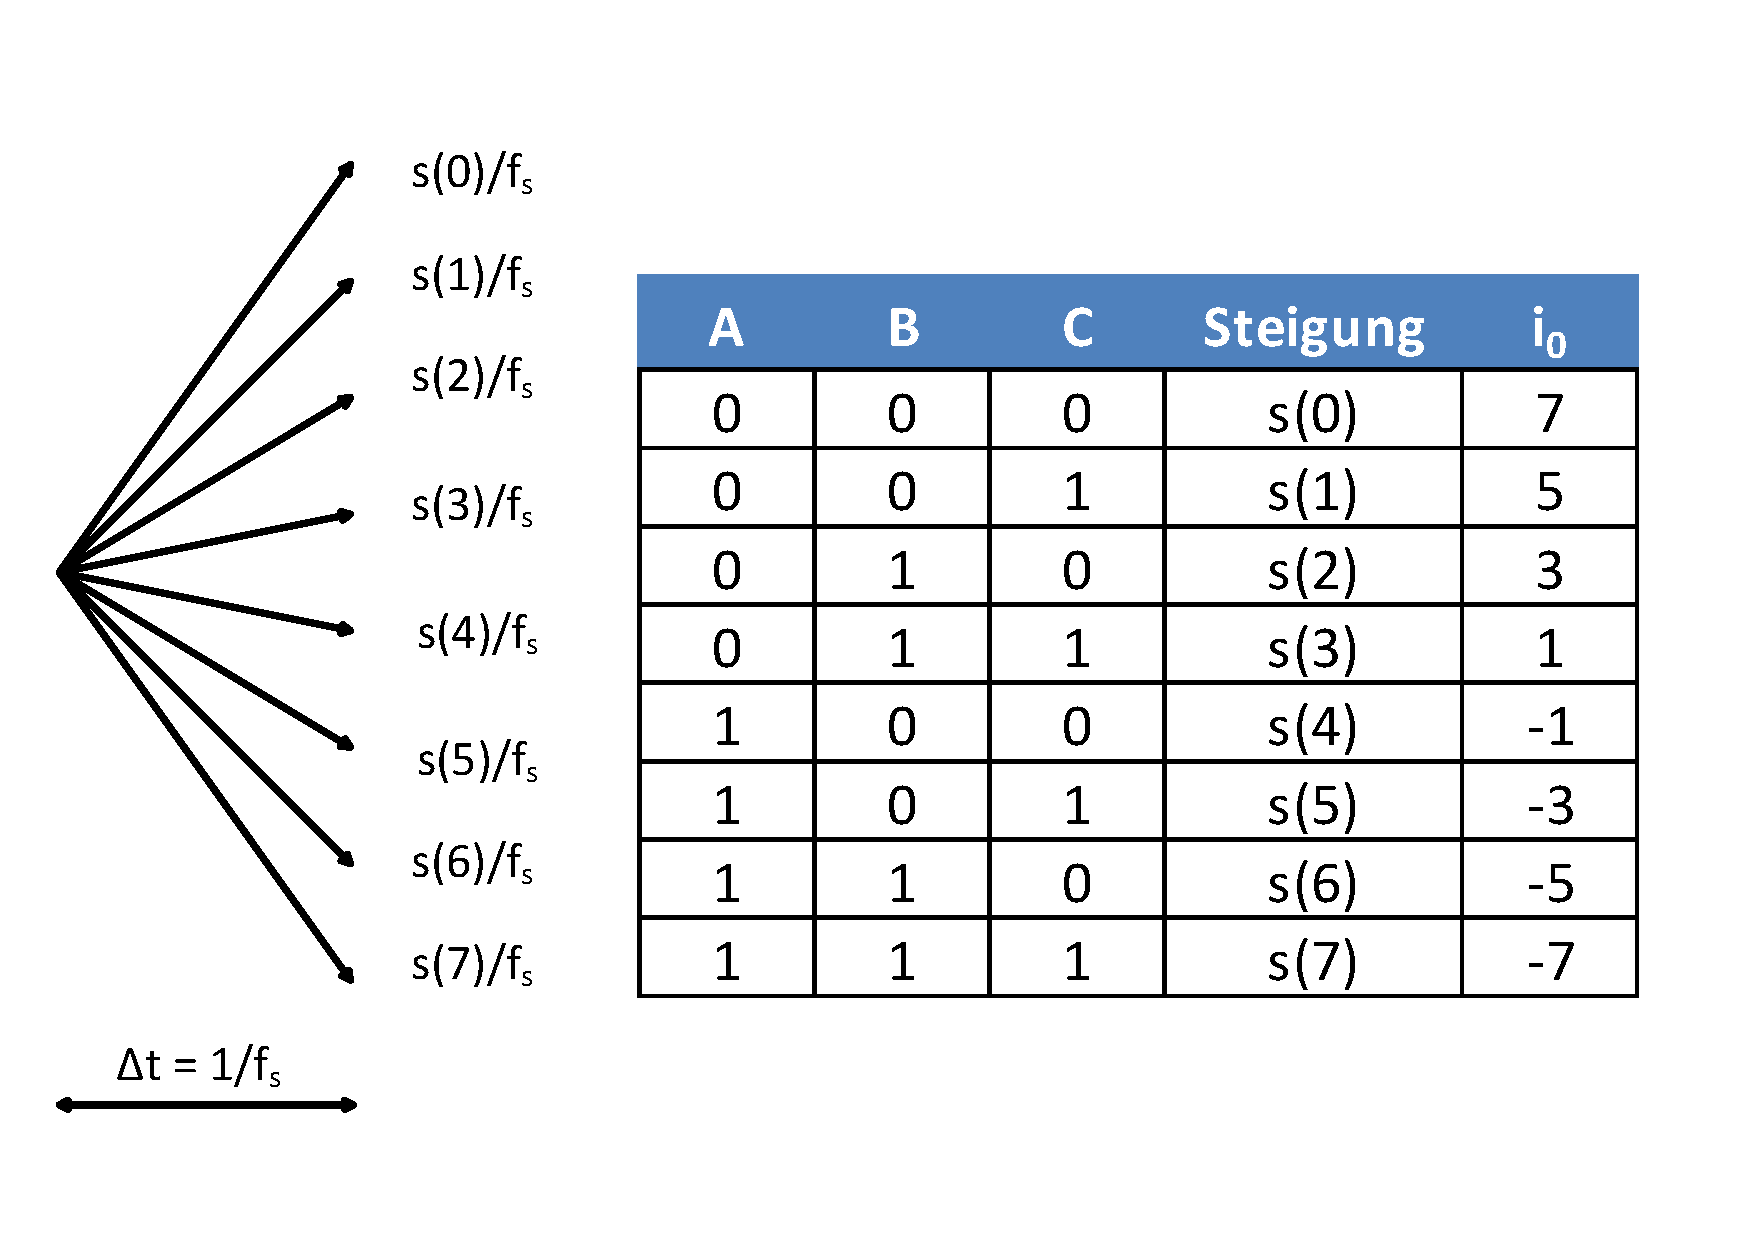
\includegraphics[width=.75\textwidth]{SlopesAndTable.pdf}
	\caption{slopes and corresponding code of the synthesized signal}
	\label{fig:SlopesAndTable}
\end{figure}

With this information a high speed digital to analog converter is created. In the following the Riemann Integral is shown.

\begin{figure}[ht]
	\centering
  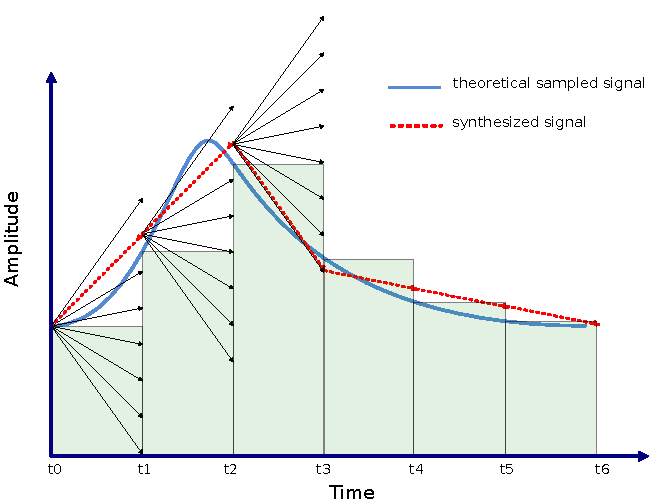
\includegraphics[width=.75\textwidth]{RiemannIntegral.pdf}
	\caption{Integral of the current which pumps charges on to the cap.}
	\label{fig:RiemannIntegral}
\end{figure}
This integral with its slopes as cited in \ref{fig:SlopesAndTable} generates the riemann code which controls the switches of the circuit. This is done by minimizing the error between the theoretical, desired signal and its synthesized one as shown in Fig. \ref{fig:RiemannIntegralError}
 \begin{figure}[ht]
	\centering
  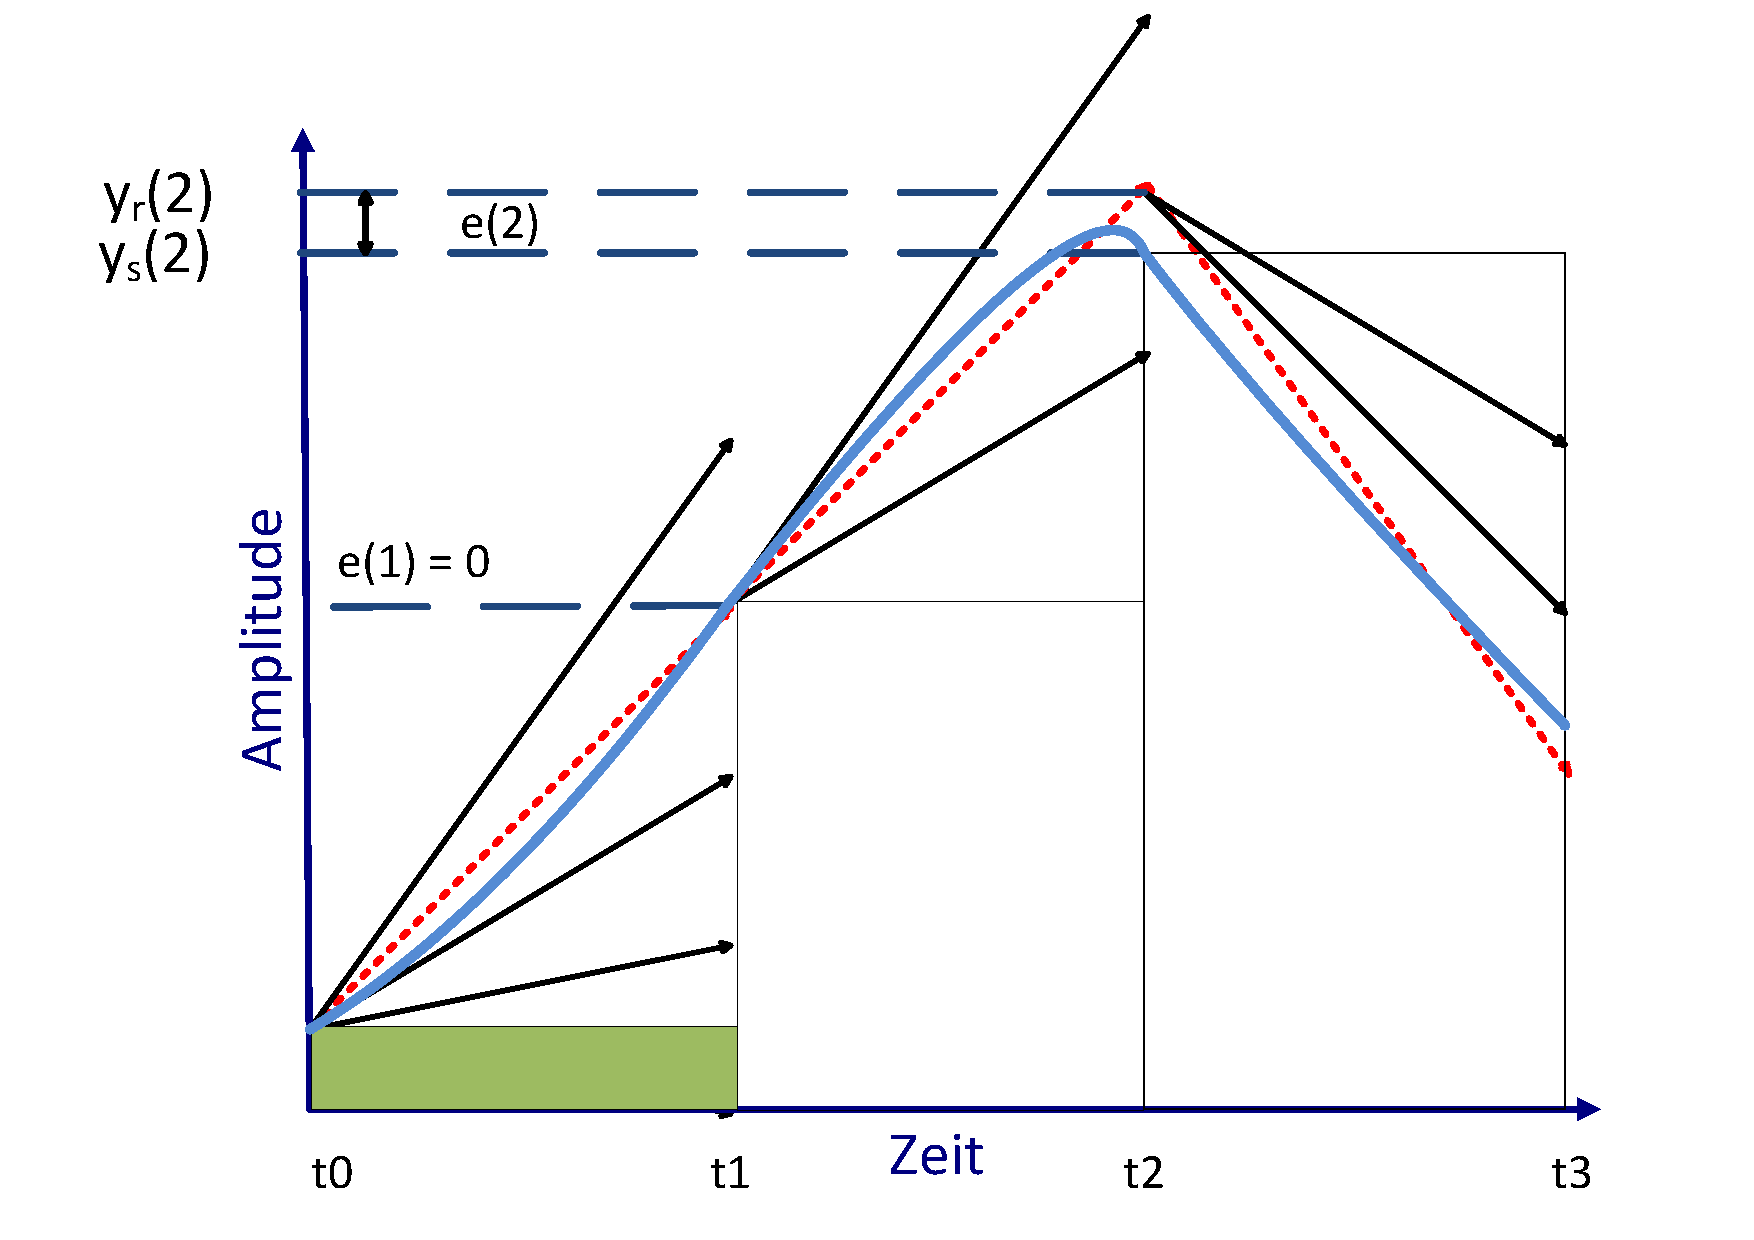
\includegraphics[width=.75\textwidth]{RiemannIntegralError.pdf}
	\caption{Code generation - error minimizing}
	\label{fig:RiemannIntegralError}
\end{figure}
The signal to noise ratio is calculated in equation \ref{eq:SNR_RiemannPumpConversion}. Quantization noise model {reference: analog device}
\begin{equation}
	\text{SNR } [\si{\dB}] = 6.02N + 9.03r - 7.78 + 10\log_{10}(1 - \frac{1}{2}^{N-1} + \frac{1}{2}^{2N})
	\label{eq:SNR_RiemannPumpConversion}
\end{equation}

\textbf{Description of the OSR, Nyquist-Shannon theorem and the SQNR...}
The \gls{ab:osr} is four and hence due to the Nyquist-Shannon theorem, the sampling \gls{sy:freq} is eight times the signal frequency.
This in mind, tuning the sampling frequency will result in tuning the signal frequency.
\textit{introducing noise due to the conversion}
\gls{ab:sqnr}
The deviation of the two signals is lying in the nature of converting digital to analog in form of quantization noise.

\section{Characteristics of Digtial-to-Analog converter}
\label{ch:characteristics}
The characteristics of different digital to analog converter are the generation of noise in terms of signal to (quantization) noise ratio.
This snr give a good insight to the performance of the corresponding dac without a focus on energy consumption nor efficiency.
\textit{Explain the different SNR (short), display the table to compare them.}


\section{summary - evaluation}
Evaluation of the idea. In the next chapters a proof of concept is done. What are the drawbacks, advantages and disadvantages.
